\documentclass{article}

\usepackage{amsmath}
\usepackage{amssymb}

\usepackage{graphicx}

\title{A sutdy of the Runge-Kutta method:}
\author{Clement Twumasi, Mehmet Cadirci and Alvaro Torras.}

\begin{document}
    \maketitle
    In this project we will be studying the following system of ODEs.
    $$
    \begin{cases}
        \dfrac{dx}{dt} = \sigma (y - a) \\
        \dfrac{dy}{dt} = a (\rho - z) - y \\
        \dfrac{dz}{dt} = a y - \beta z.
    \end{cases}
    $$
    Which we ploted on figure \ref{fig:lorentz_attractor}
    \begin{figure}[!hbtp]
    \begin{center}
        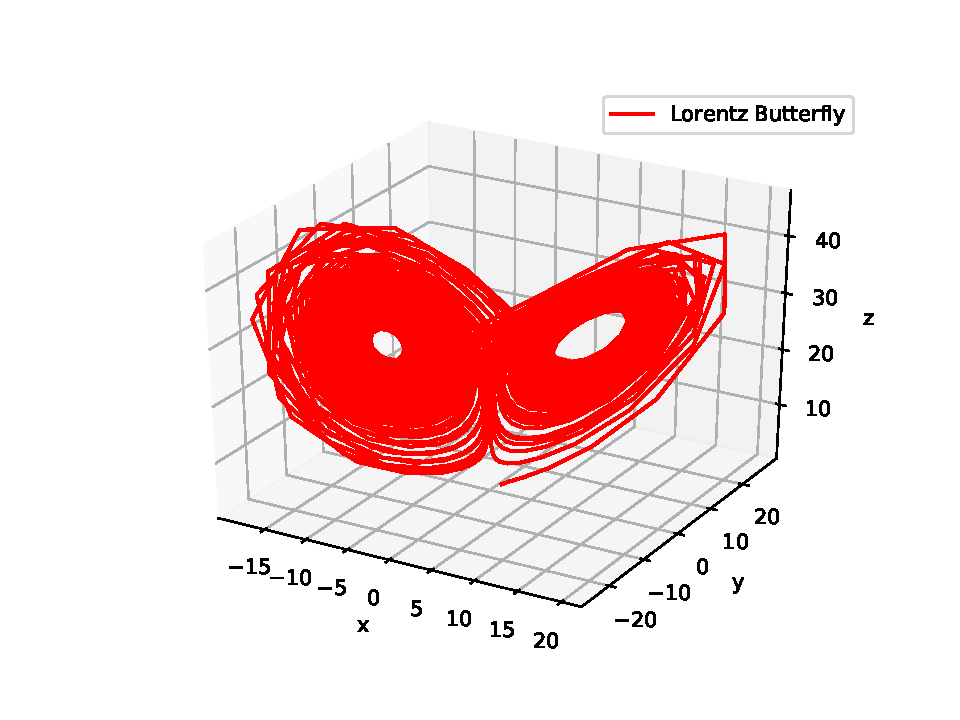
\includegraphics[width=5cm]{src/buterfly.pdf}
        \caption{Lorentz attractor.}
        \label{fig:lorentz_attractor}
    \end{center}
\end{figure}
\end{document}
